
\documentclass[journal]{IEEEtran}

\usepackage{graphicx}
\usepackage[utf8]{inputenc}




\begin{document}

\title{\textbf{loss weighting for learnability imbalance in multiclass-classification}}



\author{Theodor Peifer
        \linebreak
        email: thp7219@thi.de
        \linebreak
        Technische Hochschule Ingolstadt
}



\maketitle


\begin{abstract}
Neural Networks have proven themselves to be powerful classification
tools by solving problems in a range of domains with high accuracy.
Yet this accuracy is never evenly distributed across all classes, which means that the true-positive rates of each class separately are different.
This can happen even in balanced datasets since some classes are more difficult to learn by the model than others (this phenomenon is further referred to as \emph{learnability-imbalance}).
A common way to address this problem is to give a weight to the error function for each class to penalize losses of certain classes higher or lower.
This research will address the determination of such weights to counteract the learnability-imbalance in balanced datasets using previously calculated evaluation scores.
Therefore the goal is to find methods to lower the variance of the true positive rates of each class.
\end{abstract}


\section{Introduction}
A frequent problem in classification appears when working with a dataset that has an unequal amount of samples per class.
This imbalance leads the model to learn the patterns of a class with less elements worse than others.
In order to prevent this, it is common to weight the error function [1] according to the size of each class, i.e. the number of samples it contains.
Therefore, for every class there is a weight, which is greater the fewer elements it contains and that gets multiplied with the loss produced by its samples.
Since the aim of a neural network is to minimize the overall loss and samples from a smaller class will produce a higher error, they will have a higher impact on the learning process.

% , samples from that produce a high loss will have a higher impact on the learning process.
% This can prevent the model from learning the patterns of a class with less element worse than others.
% With the evaluation a set of true positive rates can be calculated for each class which reveals what classes are more difficult to learn by the model and should have received a higher weight. 

But this learnability imbalance appears also in balanced datasets for a vareity of reasons, for example when the quality of the data of a class is lower than the rest of the data. 
A second reason, that will be presented later on, is that when the two classes are similiar, 
the model can confuse their samples with each other what will often result in a lower accuracy of both classes. 
The question arises how to create loss weights for a model that gets trained on a balanced dataset. 
When working with such datasets the learnability differences of the individual classes are mostly only identifiable after the model has been trained and evaluated normally.
A confusion matrix or the calculation of the true positive rates then reveal what classes where learned the best and which should have received a higher weight.
The figure 1 below shows the true positive rates of a an evaluated convolutional neural network [2] that was trained on the CIFAR-10 dataset, which contains 32$\times$32 RGB images of ten different classes [3].
This dataset is a good show case for the learnability imbalance problem since it contains similiar classes, such as \emph{dog} and \emph{cat} and will be used as one of the main datasets to run the research experiments on.
 
\begin{figure}[h!]
        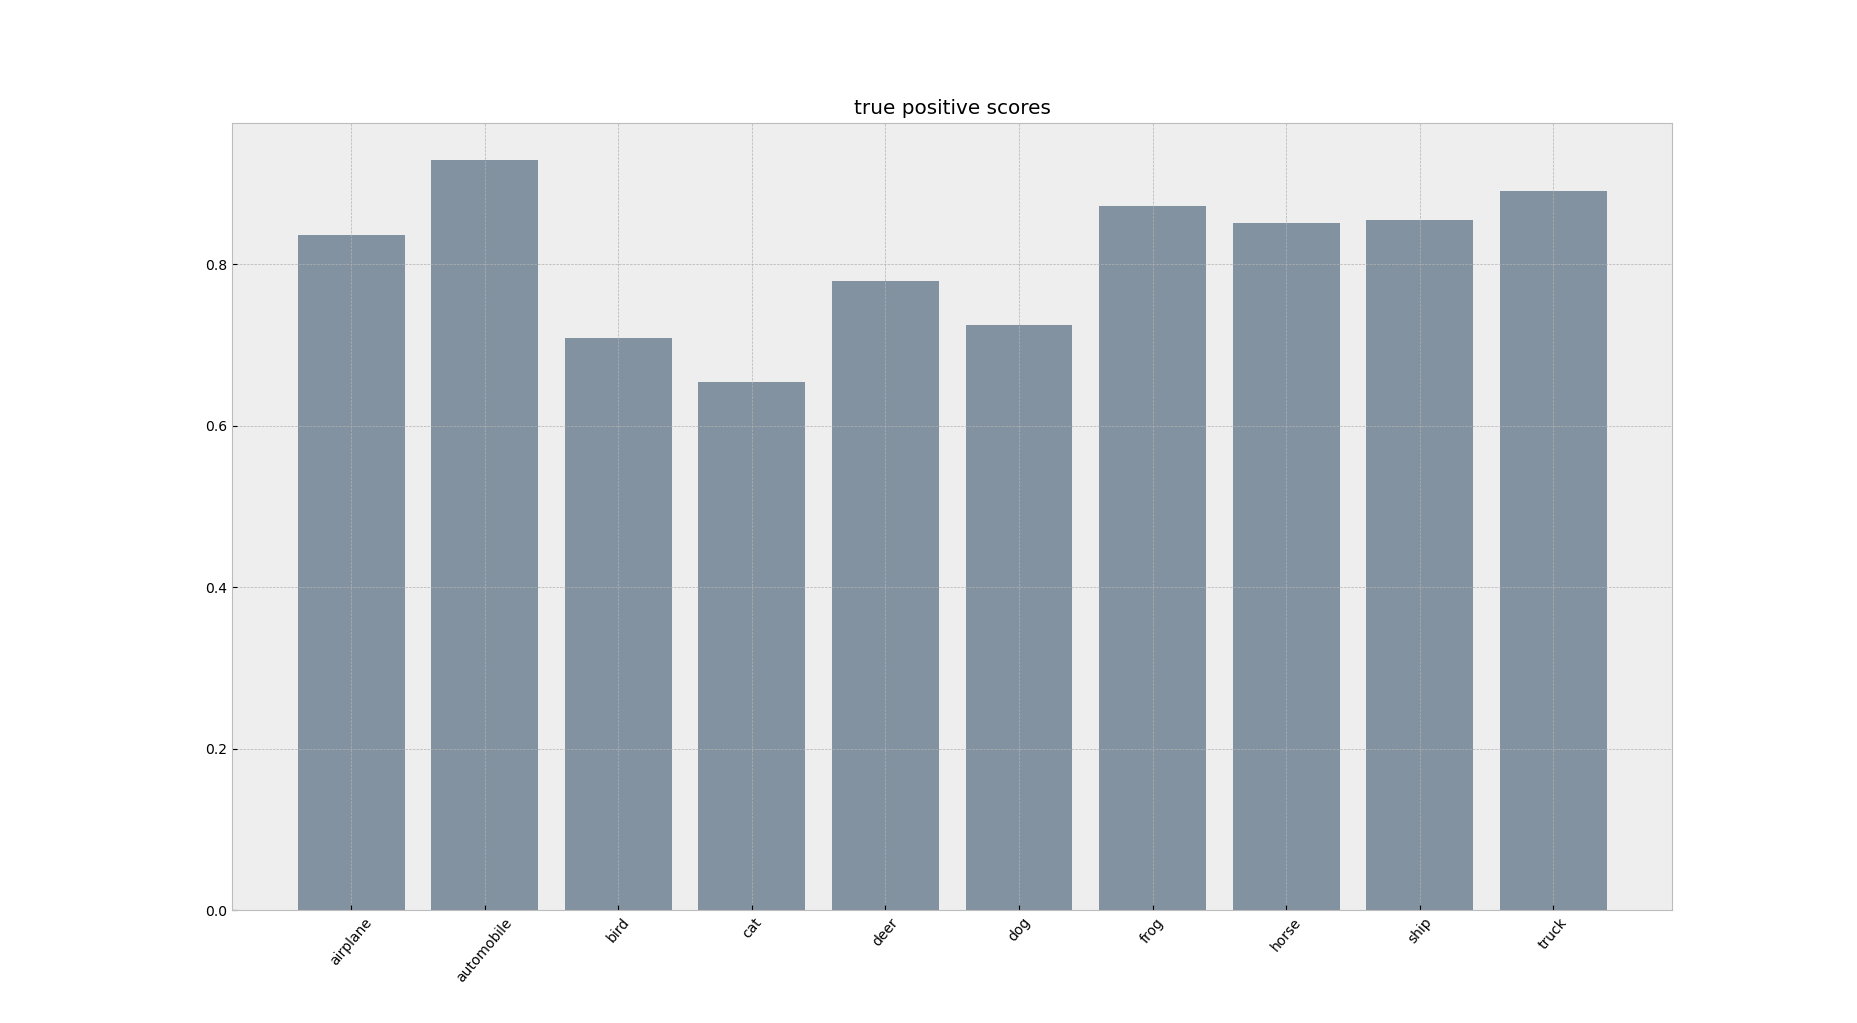
\includegraphics[width=\linewidth]{images/cifar10_tp_scores.png}
        \caption{true positive scores of a model trained on the CIFAR-10 dataset}
        \label{fig:tp_scores}
\end{figure}
% Figure \ref{fig:tp_scores} shows true positive scores.

Looking at the true positive rates it can be seen that there are some classes that got misclassified more often (in this case bird, cat deer and dog). 
Since this dataset is mostly used to present experimental results and is, due to its small sample dimensions, a more simple classification task, 
such a variance in the evaluations scores mostly doesn't matter. But when it comes to datasets that a model has to be trained on for a real world usecase 
it is optimal to have a fair and unbiased class distribution. An example in natural language processing [4] is \emph{name-ethnicity classification} 
where a model predicts the ethnicity of a name only by its letters [5]. Names from nationalities that speak the same language (e.g. british and american) result in a lower accuracy
which therefore can lead to wrong interpretations when the model is used for social sciences experiments. The figure 2 shows a low accuracy for the \emph{british} class which comes
especially from the presence of the similiar \emph{american} class.
Therefore, additionally to the CIFAR-10 dataset, experiments on how to counteract learnability-imbalance will also be done on a name-nationality dataset using a recurrent neural network architecture [6].

\begin{figure}[h!]
        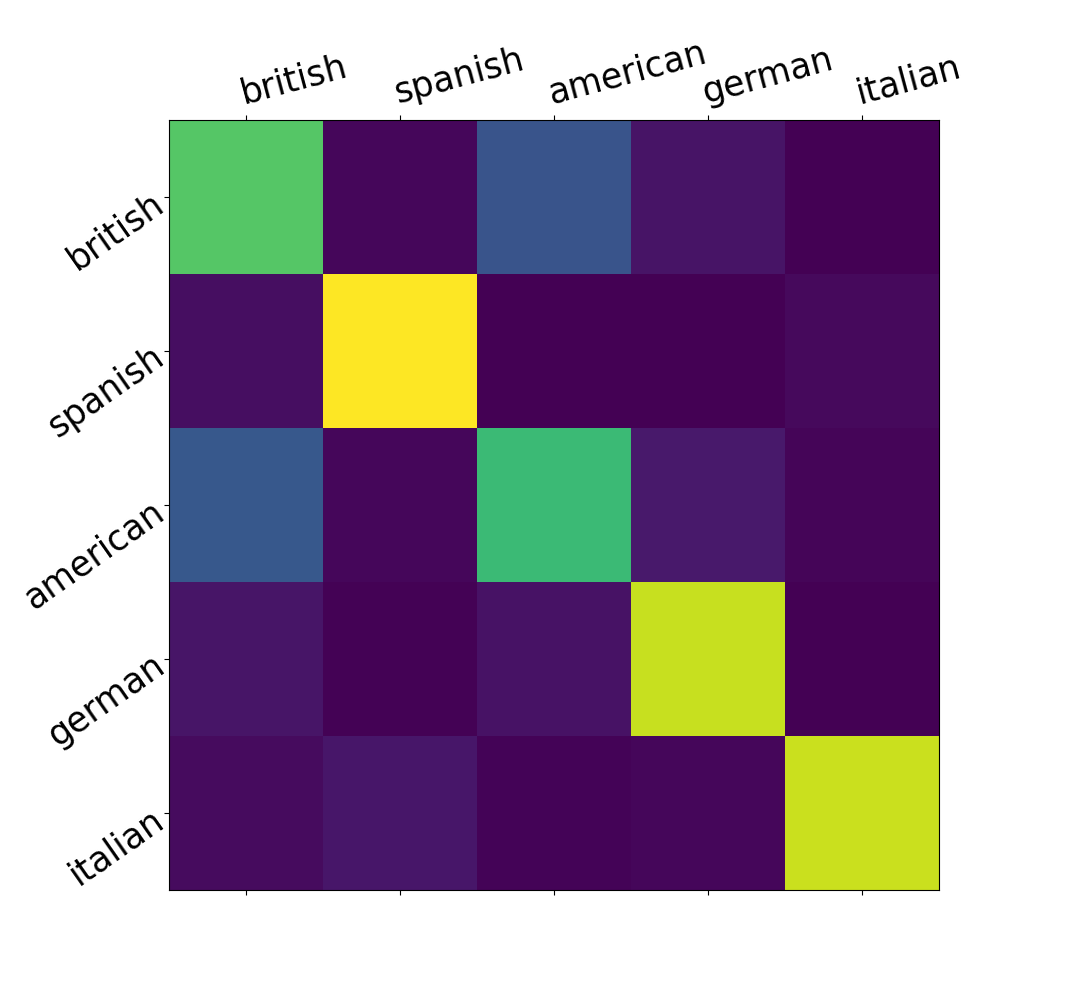
\includegraphics[width=\linewidth]{images/nec_confusion_matrix.png}
        \caption{true positive scores of a model trained on the CIFAR-10 dataset}
        \label{fig:tp2_scores}
\end{figure}

\section{state of the art}
TODO first section here


\section{approach}
TODO second section here


\section{third section}
TODO third section here


\begin{thebibliography}{1}

\bibitem{}
Name Name, Name Name, Name Name (2006). Title, 24(1), 29-33.

\end{thebibliography}


\end{document}

% biased class distribution: https://link.springer.com/chapter/10.1007/3-540-44795-4_45#:~:text=Labeled%20data%20for%20classification%20could,optimal%20classification%20on%20new%20data.